%%
%% This is file `chapall.tex',
%% generated with the docstrip utility.
%%
%% The original source files were:
%%
%% ths.dtx  (with options: `chapmin,addfig,addtbl,addbib,addglo')
%% 
%% IMPORTANT NOTICE:
%% 
%% For the copyright see the source file.
%% 
%% Any modified versions of this file must be renamed
%% with new filenames distinct from chapall.tex.
%% 
%% For distribution of the original source see the terms
%% for copying and modification in the file ths.dtx.
%% 
%% This generated file may be distributed as long as the
%% original source files, as listed above, are part of the
%% same distribution. (The sources need not necessarily be
%% in the same archive or directory.)


 %% ... sample chapter ...

The code was implemented

\section{Vector Flattening}

Data is stored as \texttt{std::vector<>} objects.

Figure~\ref{fig:indx_ex} gives an example of the spatial indexing scheme using an $8 \times 8 \times 8$ mesh. The indicated voxel has $i_x$, $i_y$, and $i_z$ indices of 1, 5, and 6 respectively. Therefore, the index value of the highlighted voxel is $1 \times 8 \times 8 + 5 \times 8 + 6$ = 110.

\begin{figure}[tb]
  \begin{center}
   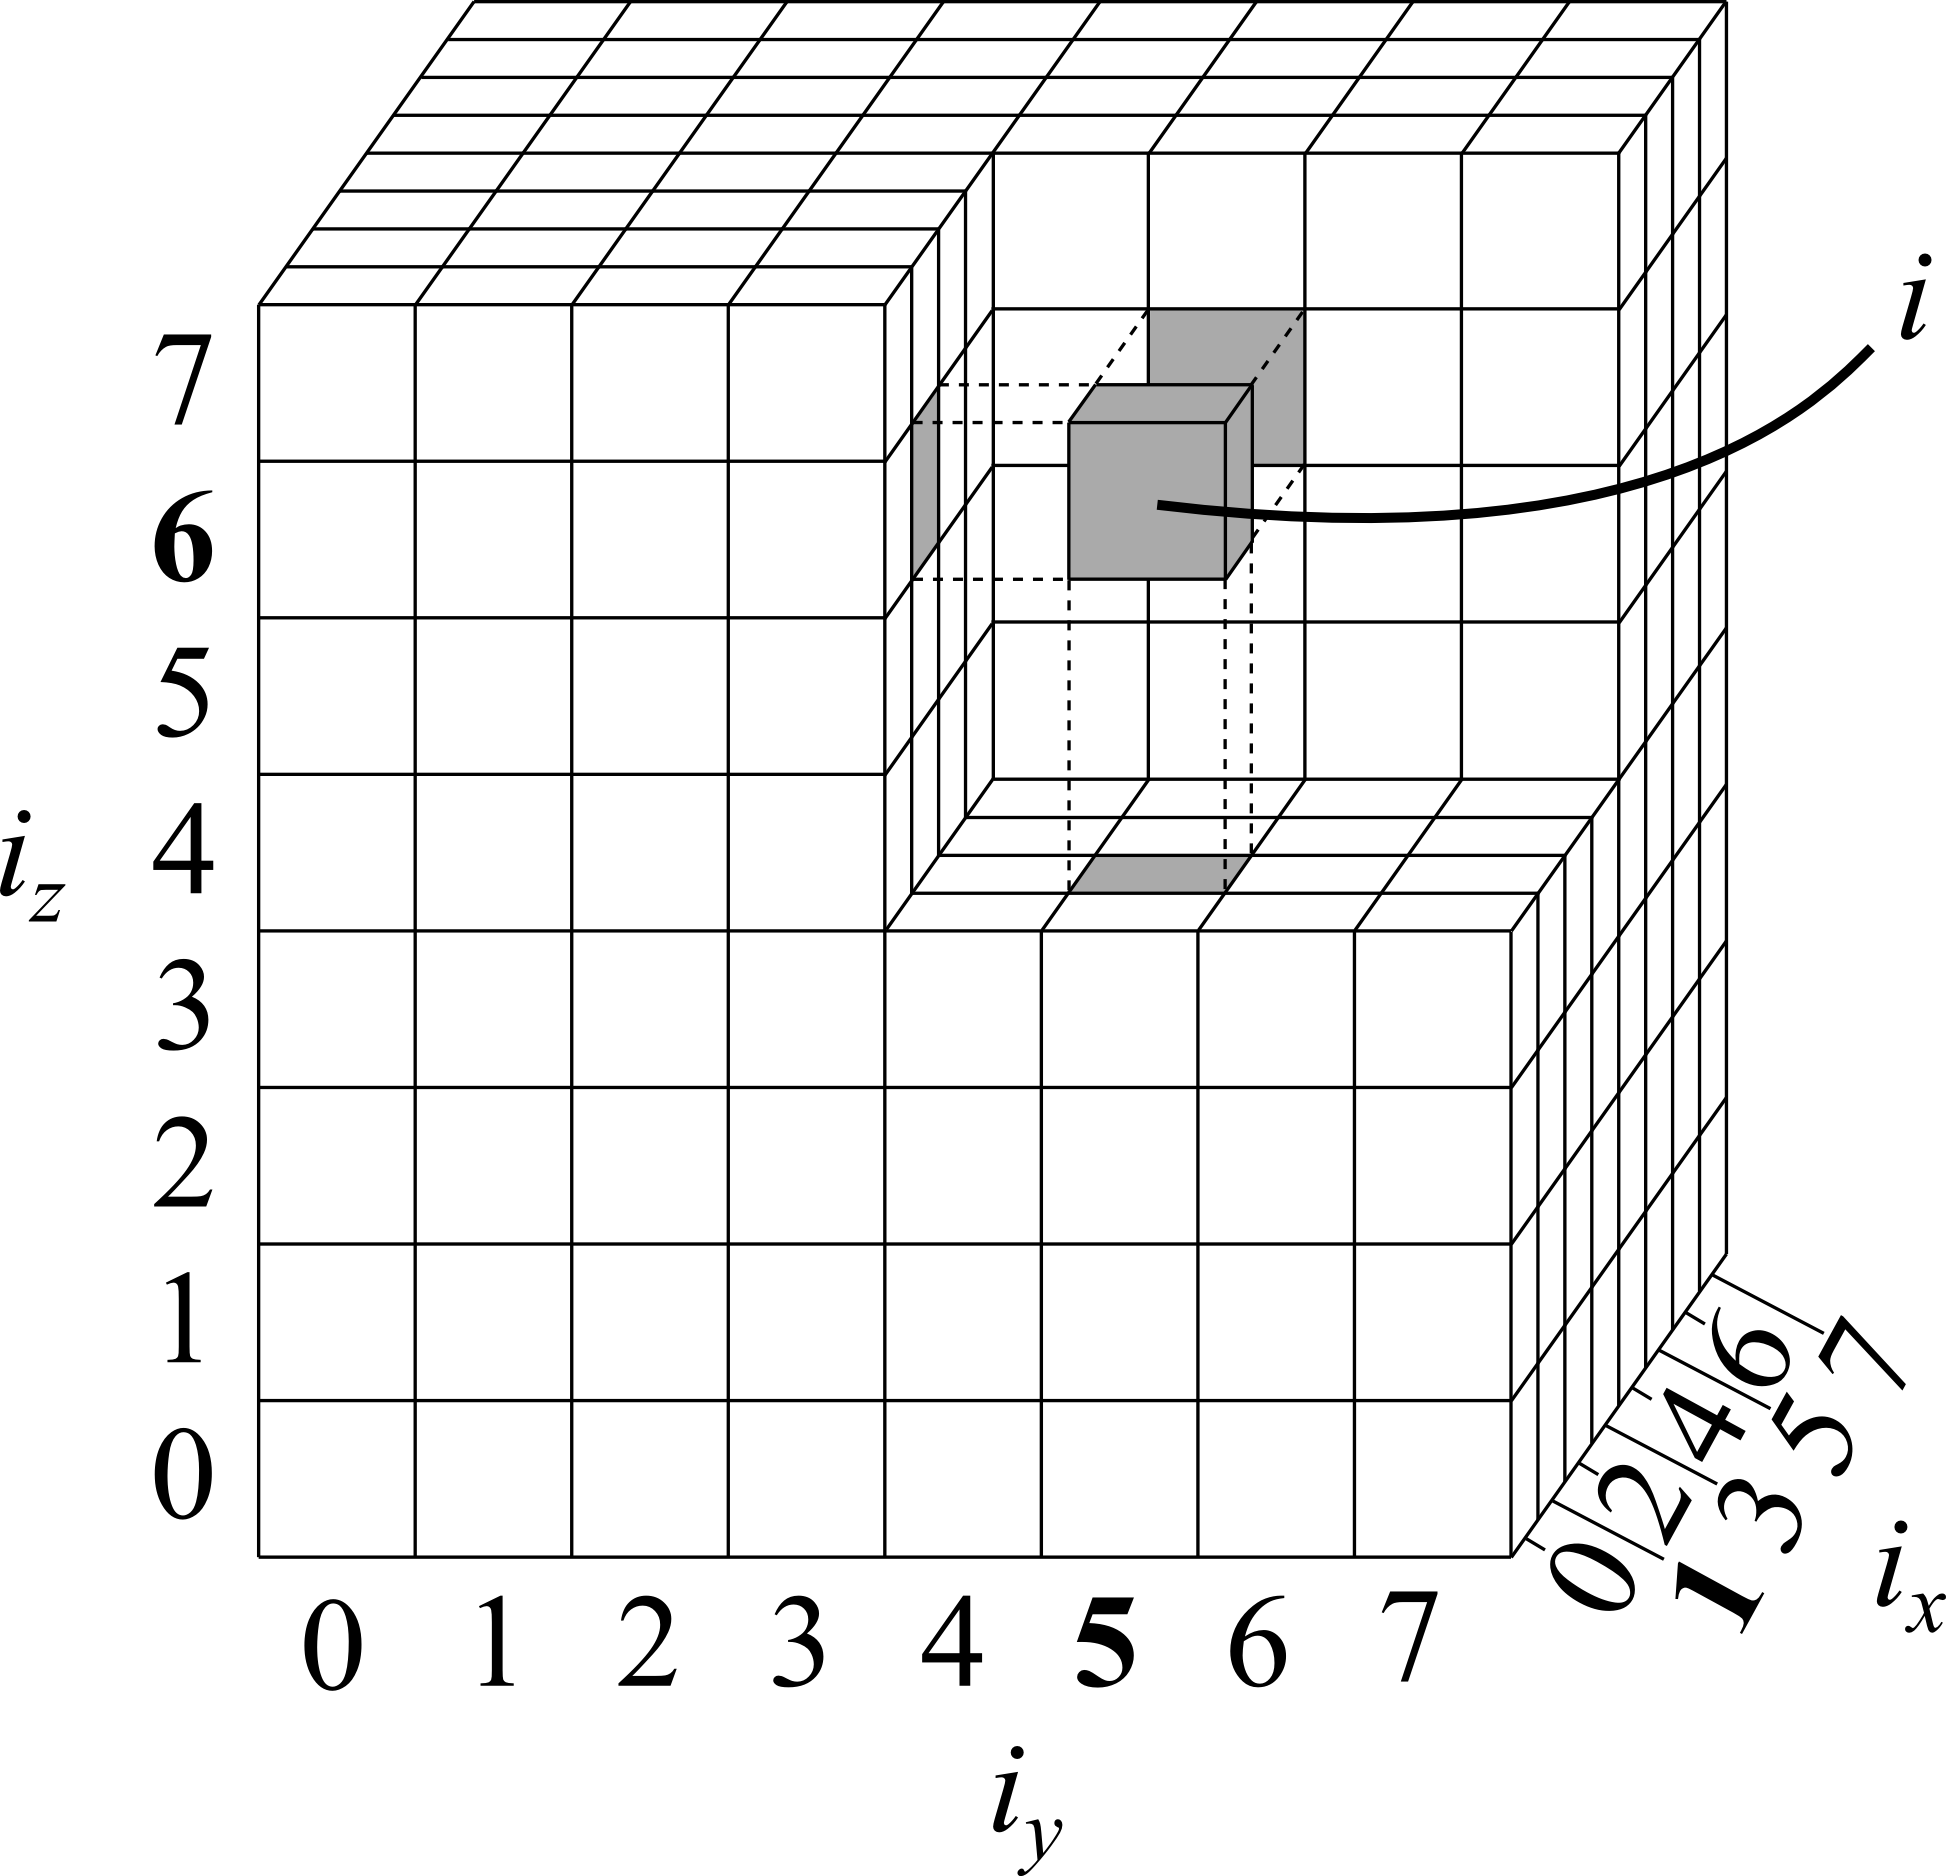
\includegraphics[width=3.75in]{figs/indx_ex}
  \end{center}
  \caption{The indexing scheme.}
\label{fig:indx_ex}
\end{figure}%

\section{Qt5 Framework}
The Qt5 framework was used for impoementation of the user interface. Qt5 enables asynchronous calls through its ssignal/slot mechanism. A signal can be emitted which will execute all connected slots. Signals and slots can be connected manually by the user except for ones automatically generated by Qt. Qt prvides a user interface for building user interfaces. Components such a sbuttons, drop boxes, radio buttons, etc. are offered to the user. Qt makes extensive use of polymorphism. All user components inherit from the base \texttt{QWidget} class which inherits from \texttt{QObject}. Any class that utilizes the signal/sloot mechanism must extend the \texttt{QOjbect} class.

Listing~\ref{lst:sync1} gives a pseudocode snippet that has a long function that will block the user interface. A corresponding dequence diagram is given in Fig.~\ref{fig:sync1}. When the user interacts with the GUI, the writer object begins executing the \texttt{doWrite()} function. Until this function completes, the UI thread will be busy an dunable to handle additionaly user interaction or updates. This results in the GUI becoming unresponsive and potentially issuing a warning to the user from the operating system.

\begin{listing}
\begin{minted}[frame=lines,linenos]{python}
import numpy as np
def myfcn(hello,world):
   return hello*world
\end{minted}
\caption{Blah blah blah.}\label{lst:sync1}
\end{listing}

\begin{figure}[tb]
  \begin{center}
   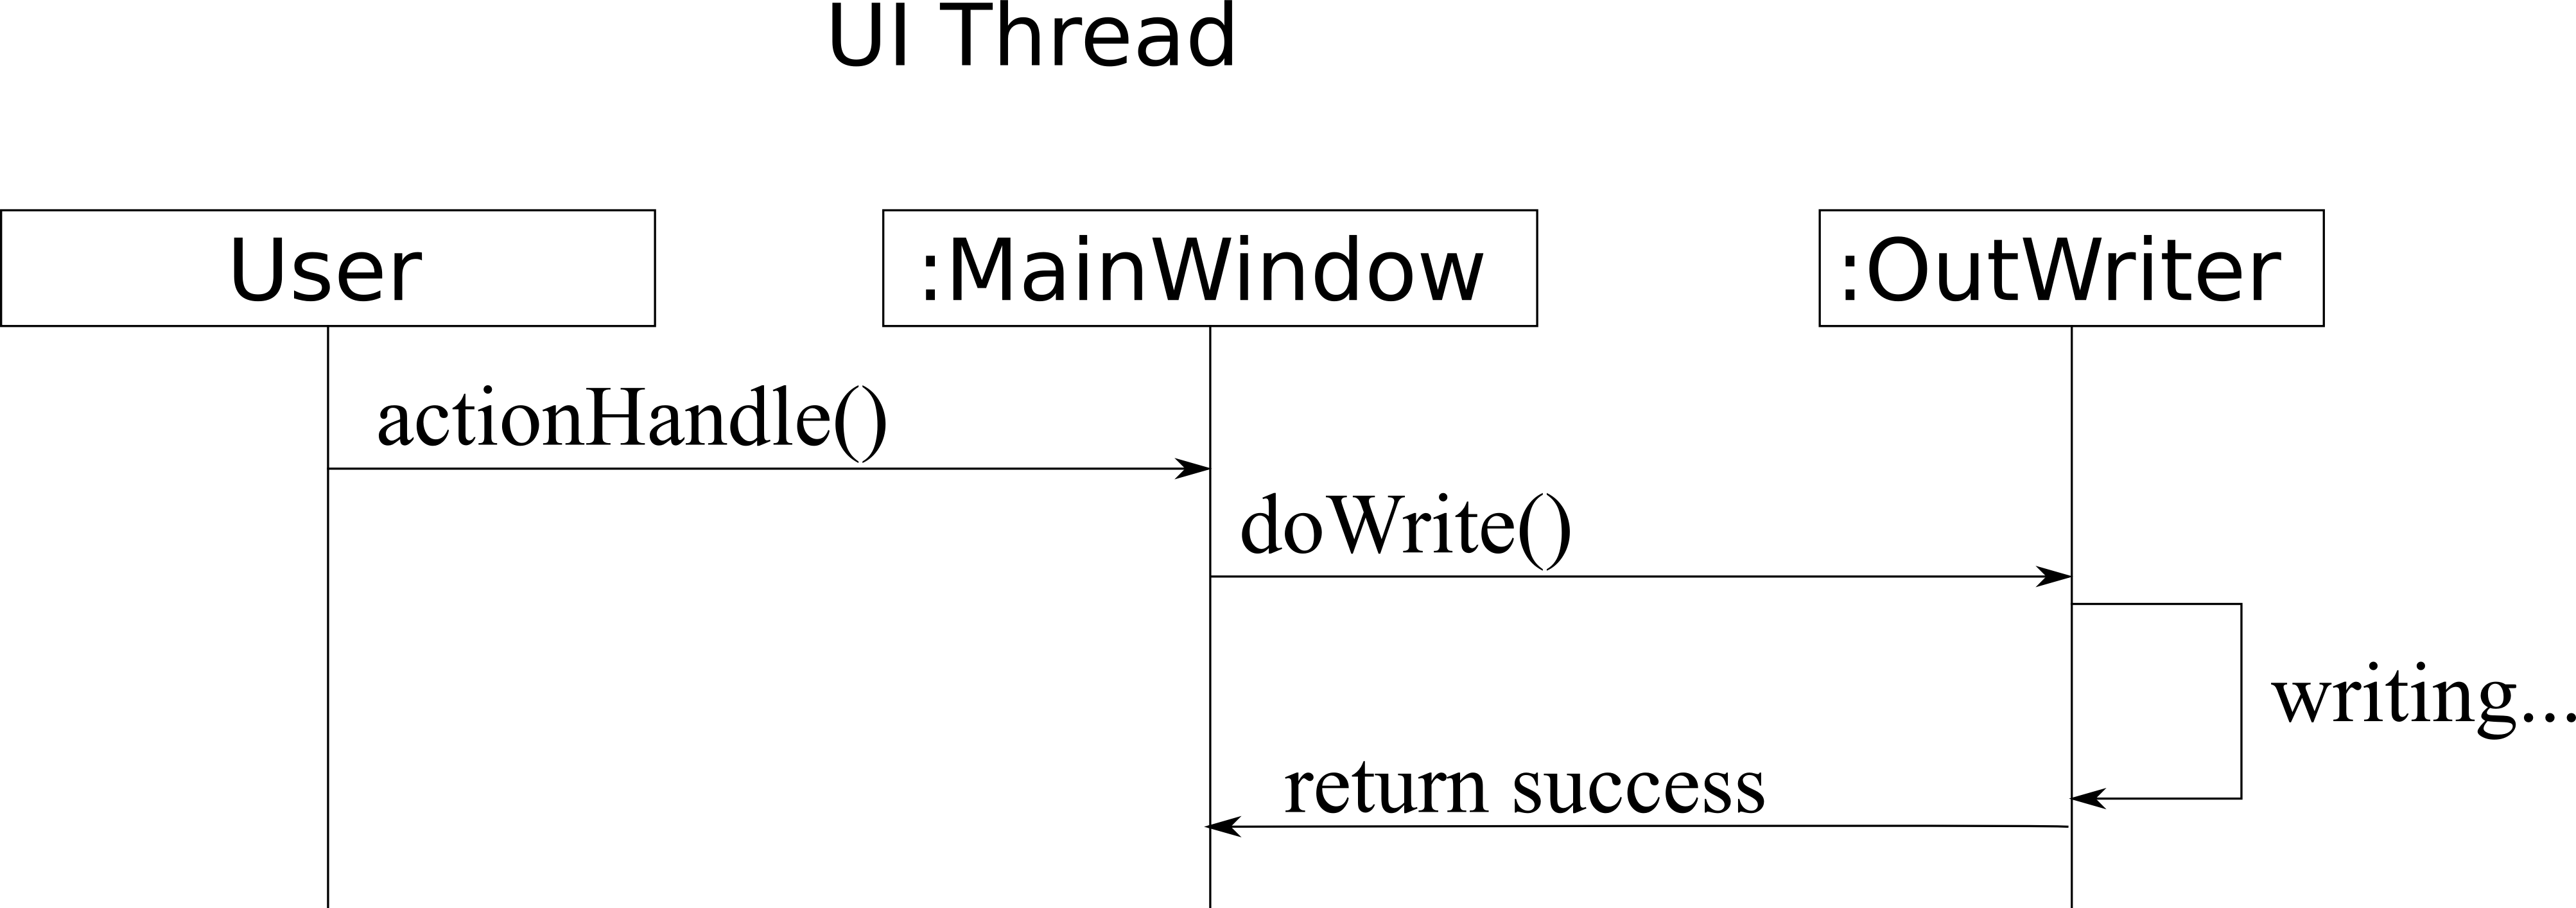
\includegraphics[width=3.75in]{figs/writer_sync}
  \end{center}
  \caption{Sequence diagram for the synchronous call.}
\label{fig:sync1}
\end{figure}%

The code in Listing~\ref{lst:sync1} is updated to use the Qt signal/slot mechanism.

\begin{figure}[tb]
  \begin{center}
   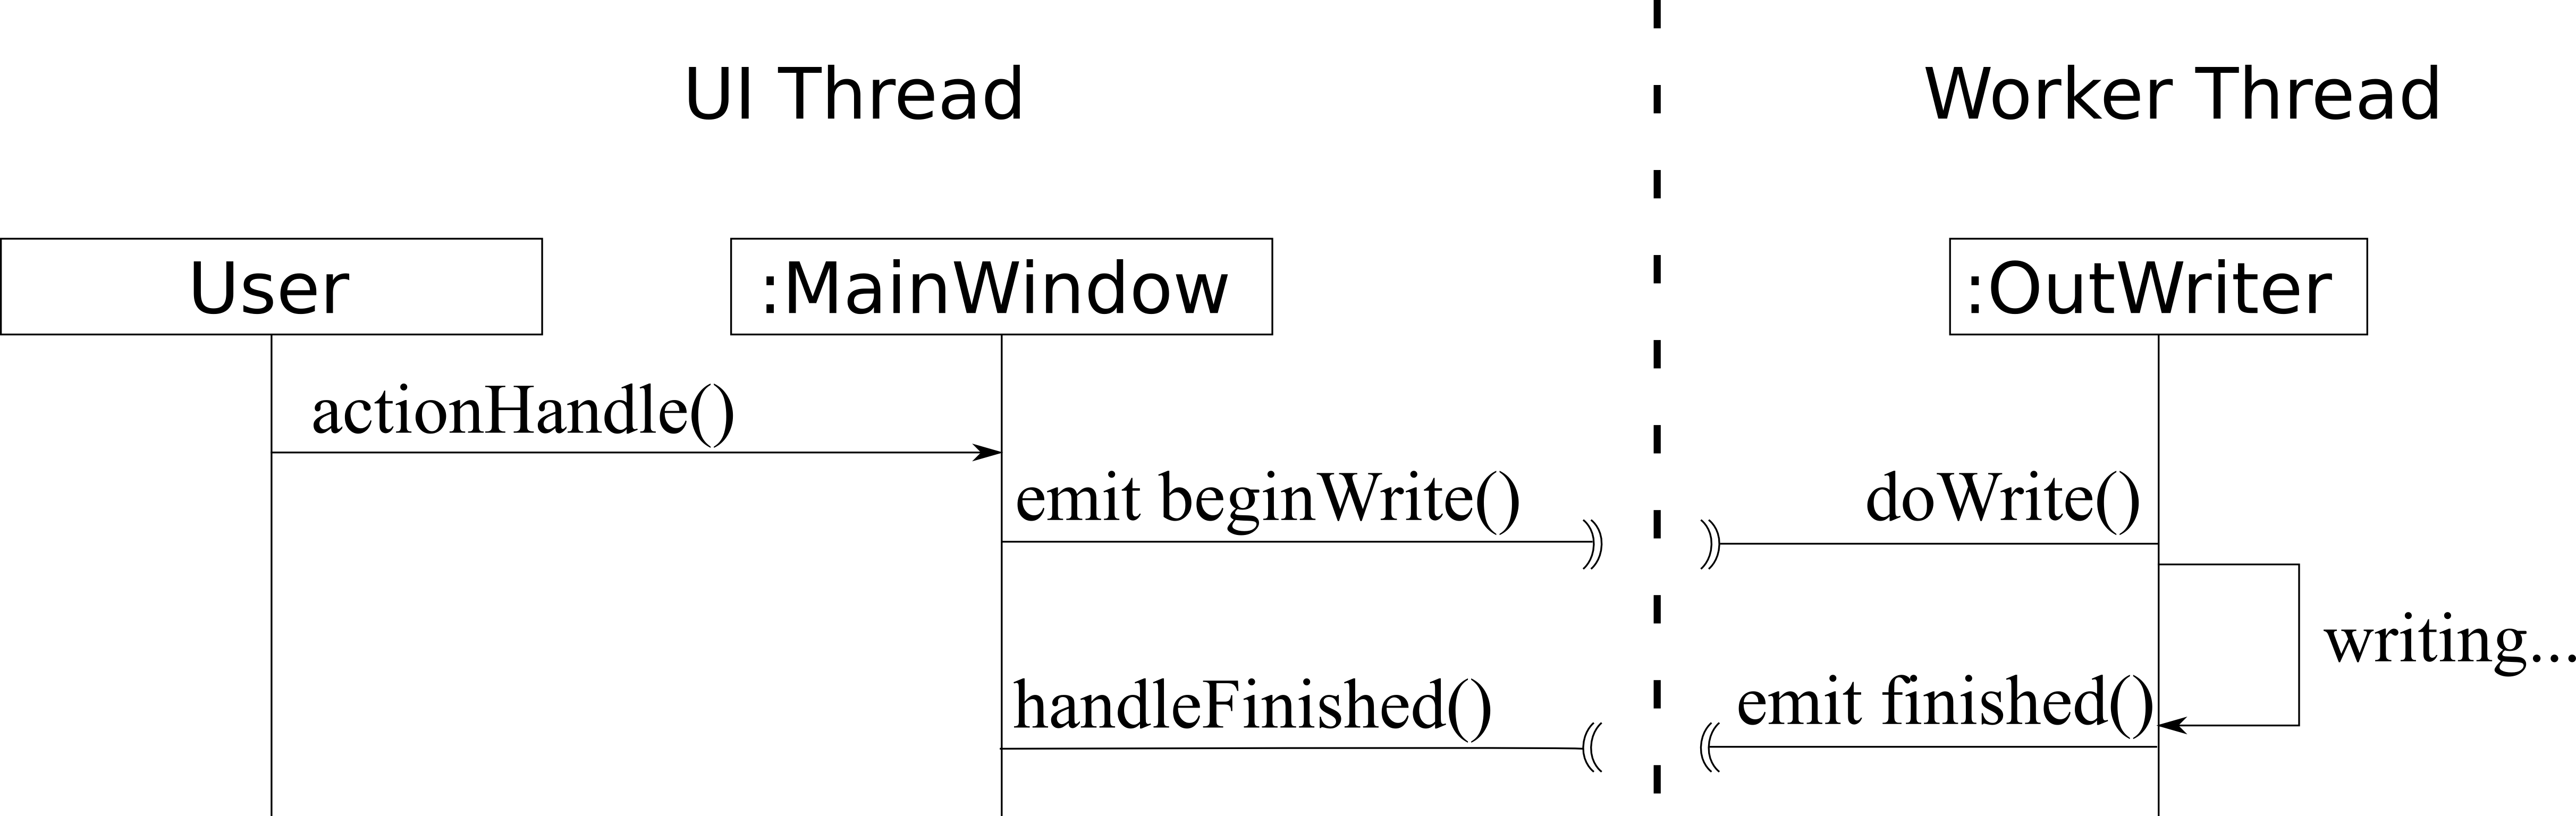
\includegraphics[width=3.75in]{figs/writer_async}
  \end{center}
  \caption{Sequence diagram for the synchronous call.}
\label{fig:async1}
\end{figure}%

\section{CUDA}
CUDA code is compoiled with the Nvidia complier nvcc. Qt uses the gcc compiler and its MOC generator for meta code. In order to connect CUDA code to the Qt MOC, the CUDA code is compiled by nvcc to produce a .o file. Qt then compiles all other files into corresponding.o files. The linker than automactically picks up all of the .o files gneerated by nvcc. The final result is an executable that has a Qt generarted user interface that can communicat with an Nvidia graphics card through the CUDA language.

The sweep through the mesh is different.

\begin{tabular}{ l | c | c | c}	
  i  & ix & iy & iz \\ \hline
  0  & 4 & 0 & 0\\
  1  & 3 & 1 & 0\\
  2  & 3 & 0 & 1\\
  3  & 2 & 2 & 0\\
  4  & 2 & 1 & 1\\
  5  & 2 & 0 & 2\\
  6  & 1 & 3 & 0\\
  7  & 1 & 2 & 1\\
  8  & 1 & 1 & 2\\
  9  & 1 & 0 & 3\\
  10 & 0 & 4 & 0\\
  11 & 0 & 3 & 1\\
  12 & 0 & 2 & 2\\
  13 & 0 & 1 & 3\\
  14 & 0 & 0 & 4\\
\end{tabular}

We first split the mesh into levels, $L$. The number of elements before the 4$^{th}$ level is 1 + 2 + 3 = 6. This is simply the sum of all integers less than the level number given by Eq.~\ref{eq:levelsum}. This is conincidentally the index of the first element of that level. However, there is a special case of $N_0 = 1$.

\begin{equation} \label{eq:levelsum}
N_L = \sum_{i=1}^{L} = \frac{L(L+1)}{2}
\end{equation}

Given an index, $i$, the level to which it belongs can be computed by substituting $i$ for $N_L$ in Eq.~\ref{eq:levelsum} and solving for $L$. The index value is then floored.

\begin{equation} \label{eq:levelquadratic}
i = \frac{L(L+1)}{2} \rightarrow L^2 + L - 2i = 0
\end{equation}

\begin{equation} \label{eq:levelquadsol1}
L = \left \lfloor{\frac{-1 \pm \sqrt{1+8i}}{2}} \right \rfloor
\end{equation}

Since the index must be a positive value, the $\pm$ sign can be removed from Eq.~\ref{eq:levelquadsol1} yielding Eq.~\ref{eq:levelquadsol2}

\begin{equation} \label{eq:levelquadsol2}
L = \left \lfloor{\frac{-1 + \sqrt{1+8i}}{2}} \right \rfloor
\end{equation}

The maximum index of any level in a the $N$ subsweep is $N$. Each subsweep adds an additional level. Therefore, the ix, iy, and iz indices can be computed using Eq.~\ref{eq:levelix},~\ref{eq:leveliy}, and~\ref{eq:leveliz} respectively.

\begin{equation} \label{eq:levelix}
ix = N - N_L
\end{equation}

\begin{equation} \label{eq:leveliy}
iy = L + N_L - i
\end{equation}

\begin{equation} \label{eq:leveliz}
iz = L + i - N_L
\end{equation}

Some examples are given in the following section
\subsection{Example 1}
In the $N=4$ subsweep, 



\section{Hardware}
For this work, a computer with an Intel i7-5960X 8 core (16 hyperthreads) processor with a base clock speed of 3.X GHz and two Nvidia Titan Z graphics cards were used. The KBA algorithm was used to map th eproblem domain onto the GPU. A second version was created taht utilized both graphics cards. Currently, if the problem requires more memory than is available on the GPU, the problem can still be solved, but much more time will be required to to copy overhead between the CPU and GPU. If the problem requires more memory than either the GPU or CPU can provide, an error is thrown and the simulation is not run.


\section{Section with \texttt{nomencl} Entries}

Finally, we add a simple equation to illustrate the use of the nomencl
 package for automatic generation of a list of symbols.
\begin{equation}
\delta_i = \sqrt{t/\mathrm{Pe}}
\end{equation}
where $\delta$ is the layer
thickness %
\nomenclature[at]{$t$}{time}%
\nomenclature[gd]{$\delta$}{layer thickness}%
\nomenclature[si]{$i$}{inlet}%
as defined previously. \lipsum[26-30]

\endinput
%%
%% End of file `chapall.tex'.
